\section{Latch Etapa de decodificaci\'on - Etapa de ejecuci\'on}

\subsection{M\'odulo}
Este latch se encarga de mantener en un ciclo de clock las senales que salen de la etapa de decodificaci\'on y pasan a la etapa de ejecuci\'on. Ver figura \ref{fig:Latch}.

\begin{figure}[H]
\centering
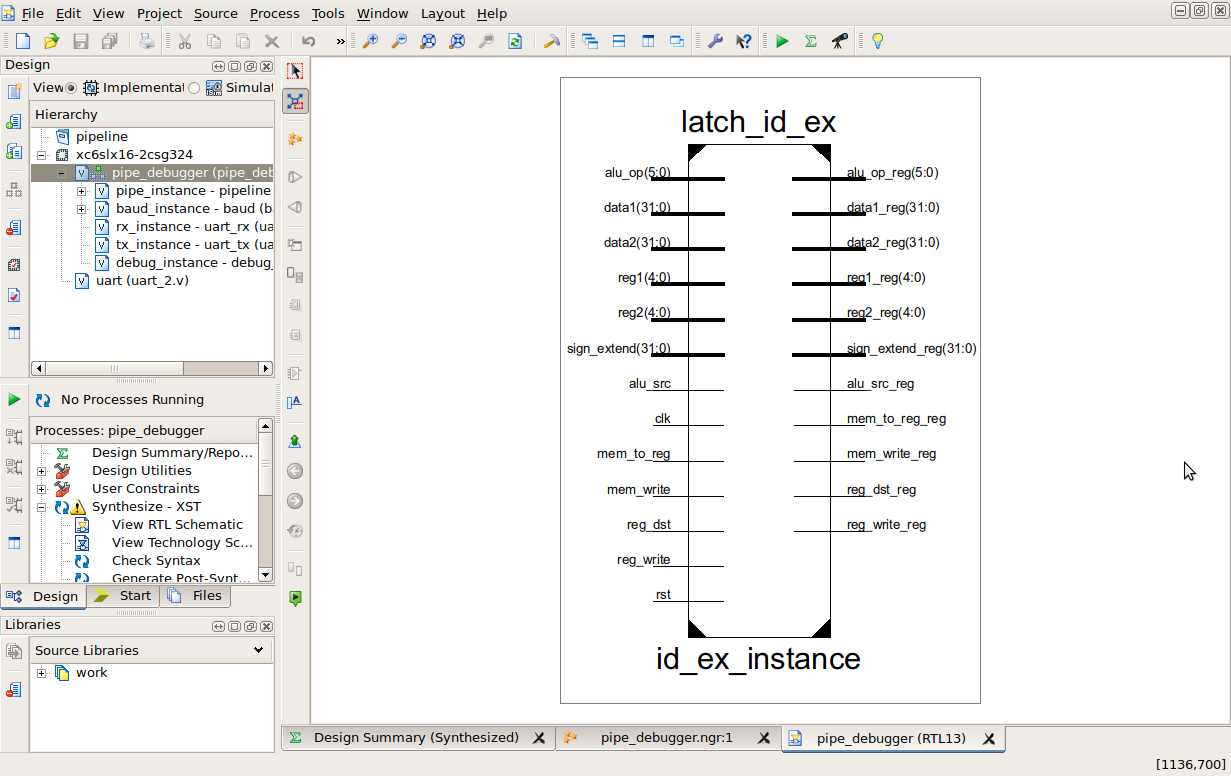
\includegraphics[scale=0.5]{img/latch_id_ex}
\caption{Latch Etapa de decodificaci\'on - Etapa de ejecuci\'on}
\label{fig:Latch}
\end{figure}

Este m\'odulo tiene como entradas:
\begin{itemize}
  \item \textbf{alu\_op}: Bus de 6 bits que contiene el opcode que descifra la alu para conocer que operaci\'on debe ejecutar.
  \item \textbf{data1}: Bus de 32 bits que contiene el dato que se obtiene del banco de registros.
  \item \textbf{data2}: Bus de 32 bits que contiene el dato que se obtiene del banco de registros.
  \item \textbf{reg1}: Bus de 5 bits que contiene el puntero al registro 1 seleccionado.
  \item \textbf{reg2}: Bus de 5 bits que contiene el puntero al registro 2 seleccionado.
  \item \textbf{sign\_extended}: Bus de 32 bits que contiene el valor del dato de las instrucciones inmediatas de 16 bits extendidas a 32 bits con o sin signo.
  \item \textbf{alu\_src}: Cable que va a un multiplexor en la etapa de ejecuci\'on que elige que tipo de dato va a entrar a la alu. 
  \item \textbf{clk}: Clock general del sistema.
  \item \textbf{mem\_to\_reg}: Cable que se activa en caso de que se deban mover datos de memoria hacia registros.
  \item \textbf{mem\_write}: Cable que se activa en caso de que se vaya a escribir en la memoria de datos.
  \item \textbf{reg\_dst}: Cable que se activa y llega a un multiplexor para decidir que registro se va a elegir para escribir.
  \item \textbf{reg\_write}: Cable que entra en el banco de registros y le indica si debe o no escribir alguno de los 32 que posee.
\end{itemize}

Las salidas son las mismas entradas demoradas un ciclo de reloj.

\subsection{TestBench}
TBD